\documentclass[fleqn]{article}

\usepackage{graphicx}
\usepackage{xurl}
\usepackage{url}
\usepackage{caption}
\usepackage{fancyhdr}
\usepackage{mathtools}
\usepackage{amsmath}
\usepackage{amssymb}
\usepackage{tikz}
\usepackage{listings}
\usepackage{xcolor}
\usepackage{float}

\definecolor{codegreen}{rgb}{0,0.6,0}
\definecolor{codegray}{rgb}{0.5,0.5,0.5}
\definecolor{codepurple}{rgb}{0.58,0,0.82}
\definecolor{backcolour}{rgb}{0.95,0.95,0.92}

\lstdefinestyle{mystyle}{
	backgroundcolor=\color{backcolour},   
	commentstyle=\color{codegreen},
	keywordstyle=\color{magenta},
	numberstyle=\tiny\color{codegray},
	stringstyle=\color{codepurple},
	basicstyle=\ttfamily\footnotesize,
	breakatwhitespace=false,         
	breaklines=true,                 
	captionpos=b,                    
	keepspaces=true,                 
	numbers=left,                    
	numbersep=5pt,                  
	showspaces=false,                
	showstringspaces=false,
	showtabs=false,                  
	tabsize=2
}

\lstset{style=mystyle}

\usepackage{xepersian}

\settextfont[BoldFont={XB Zar bold.ttf}]{XB Zar.ttf}
\setlength\parindent{0pt}

\title{

\includegraphics[width=0.4\textwidth]{sharif.png}\\
\normalsize{دانشکده مهندسی کامپیوتر}\\
\vspace{1cm}
	
\huge{آزمایشگاه طراحی سیستم‌های دیجیتال}
\\ 
\Large{گزارش آزمایش دهم}
\\
}

\author{
\\
دکتر سیاوش بیات سرمدی
\\
\\
پارسا محمدیان --- 98102284
}

\date{\today}

\begin{document}

\clearpage\maketitle
\thispagestyle{empty}

\newpage

\pagestyle{fancy}
\lhead{آزمایشگاه طراحی سیستم‌های دیجیتال}

\rhead{پارسا محمدیان}


\tableofcontents

\setcounter{page}{1}

\newpage

\section{مقدمه}

\subsection*{عنوان گزارش}
پیاده‌سازی یک پردازنده ساده
\subsection*{موضوع}
استفاده از نرم‌افزارهای طراحی به کمک کامپیوتر \footnote{\lr{CAD}} برای طراحی 
و پیاده‌سازی مدار پشته به صورت توصیف رفتاری.
\subsection*{شرح ابزارها و برنامه‌های مورد استفاده}
در این آزمایش از نرم‌افزار \lr{ISE Desgin Suite} که محصول شرکت \lr{Xilinx} است 
استفاده کرده‌ام.

\section{چارچوب نظری و شرح آزمایش}
جزئیات پیاده‌سازی به همراه کامنت در فایل 
\lr{cpu.v} 
موجود است.

\section{تست مدار}
برای تست مدار طبق خواسته دستور کار عمل شده است. دقت شود 
\lr{X} 
به صورت ماکرو تعریف شده است و با تغییر آن نتیجه عبارت متناظر محاسبه می‌شود. برای مثال برای 
\lr{$X=8$} 
داریم : 
$$
((8+23) \times 2)-12 = 31 \times 2 - 12 = 62 - 12 = 50
$$

در شکل 
\ref{test} 
مشاهده می‌شود که مدار به درستی کار می‌کند.

\begin{figure}
	\centering
	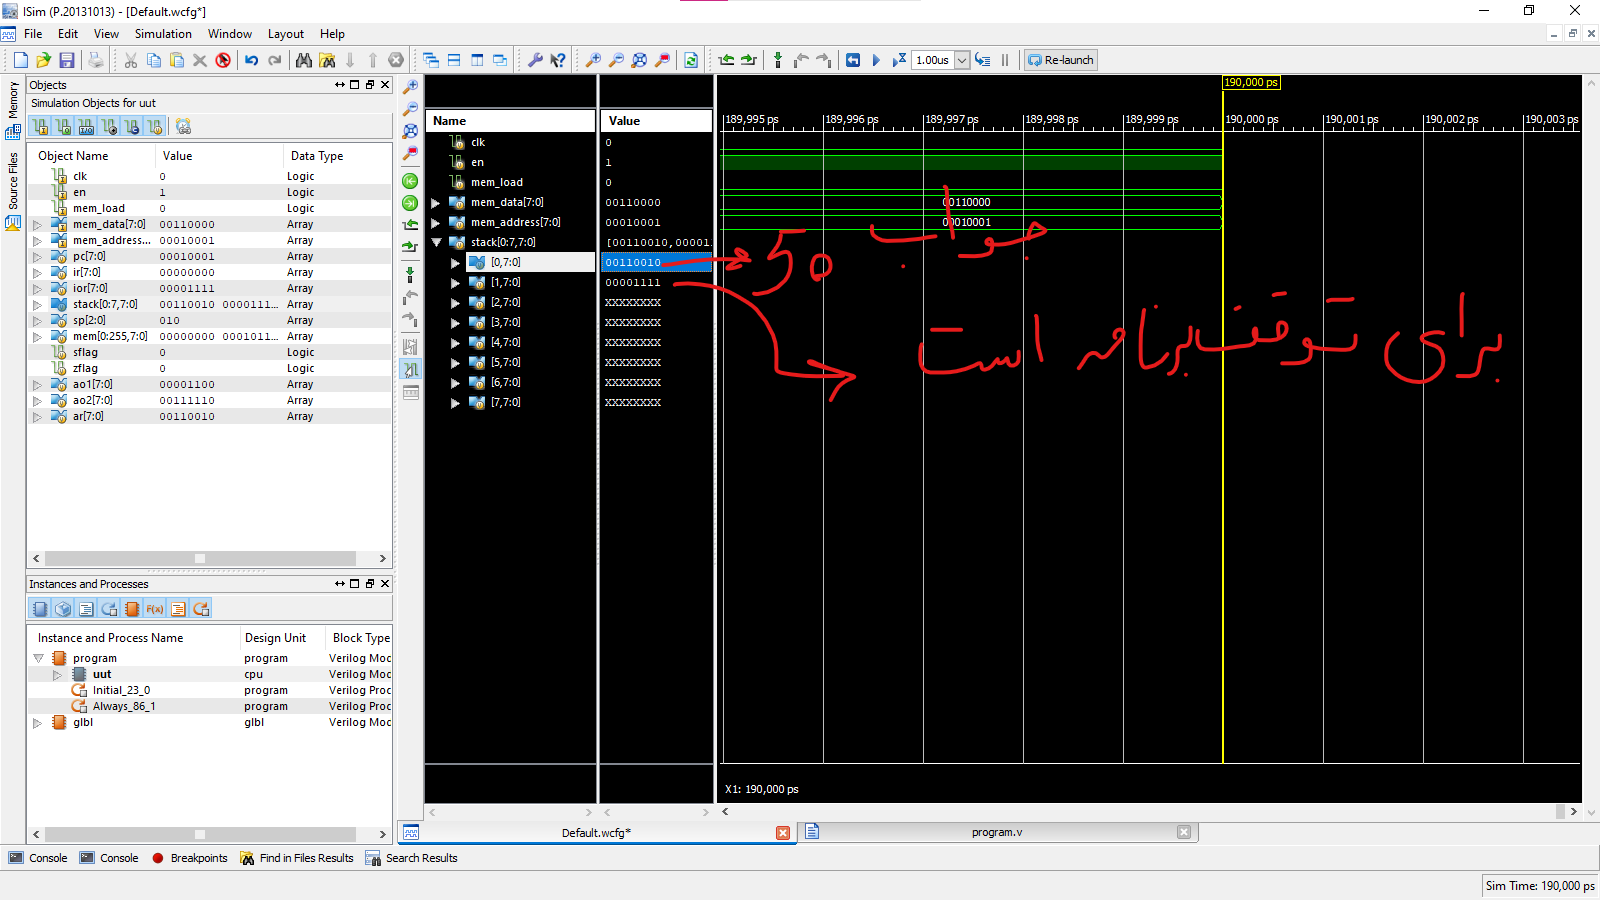
\includegraphics[width=\linewidth]{test.png}
	\caption{جواب صحیح به ازای \lr{$X = 8$}}
	\label{test}
\end{figure}

جزئیات تست در فایل 
\lr{program.v} 
موجود است. 

\end{document}
